\documentclass[a4paper]{article}

%% Language and font encodings
\usepackage[english]{babel}
\usepackage[utf8x]{inputenc}
\usepackage[T1]{fontenc}

%% Sets page size and margins
\usepackage[a4paper,top=3cm,bottom=2cm,left=3cm,right=3cm,marginparwidth=1.75cm]{geometry}

%% Useful packages
\usepackage{amsmath}
\usepackage{setspace}
\usepackage{graphicx}
\usepackage{float}
\usepackage{listings}             % Include the listings-package
\usepackage{color}

\lstdefinestyle{customc}{
  belowcaptionskip=1\baselineskip,
  breaklines=true,
  frame=L,
  xleftmargin=\parindent,
  language=C,
  showstringspaces=false,
  basicstyle=\footnotesize\ttfamily,
  keywordstyle=\bfseries\color{green!40!black},
  commentstyle=\itshape\color{purple!40!black},
  identifierstyle=\color{blue},
  stringstyle=\color{orange},
}

\lstdefinestyle{customasm}{
  belowcaptionskip=1\baselineskip,
  frame=L,
  xleftmargin=\parindent,
  language=[x86masm]Assembler,
  basicstyle=\footnotesize\ttfamily,
  commentstyle=\itshape\color{purple!40!black},
}


\usepackage[colorinlistoftodos]{todonotes}
\usepackage[colorlinks=true, allcolors=blue]{hyperref}



\title{Documentação Trabalho Prático: Twitter}
\author{Clarisse Scofield,
        Letícia Alves,
        Luiz Philippe}

\begin{document}
\begin{figure}

\includegraphics[width=0.2\textwidth]{logo-ufmg2.png}
\end{figure}

\lstset{escapechar=@,style=customc}
\maketitle



\section{Introdução}


Nossa proposta de trabalho final foi desenvolver um sistema de funcionamento semelhante à rede social Twitter. Utilizamos a linguagem C++ e as bibliotecas complementares: json (para facilitar o armazenamento dos dados) e doctest (para realizar os testes de unidade). Além disso usamos como gerenciador de versão o git com o servidor GitHub. O programa funciona no prompt de comando.

Nosso Twitter permite aos usuários enviar e receber atualizações pessoais de outros usuários. Tais atualizações, os “tweets” aparecem no feed de um usuário após ele seguir outros usuários de seu interesse.

Cada usuário, ao se cadastrar, possui seu nome de usuário (username) e sua senha (password) para fazer login no sistema. Em seu perfil, possui seus seguidores (followers), pessoas que ele segue (followees) e suas publicações (tweets). Os usuários podem interagir entre si compartilhando (retweet), respondendo (reply) ou curtindo (like) um tweet.
Pudemos assim consolidar os conhecimentos adquiridos no curso de PDS 2.

\section{Desenvolvimento}

Nosso programa é estruturado nas seguintes classes: TwitterBase, Interface, User, Tweet, Retweet, Reply e Hashtag. As funções Json serialize() e void deserialize presentes na implementação de TwitterBase, User, Tweet, Retweet, Reply e Hashtag estão relacionadas ao uso da biblioteca JSON. A primeira transforma os atributos da classe em um objeto JSON. Cada um desses objetos é salvo nos dados em um arquivo próprio. Já a “deserialize” carrega os dados do JSON para um objeto da classe. Os objetos podem ser recuperados dos dados através de um número inteiro identificador (id).

Após criar um objeto de uma das classes através de seu construtor (ou atualizá-lo), é necessário salvá-lo nos dados, o que é feito pela função bool save().
Seguindo boas práticas de programação, utilizando o princípio de encapsulamento, as classes possuem certos atributos e métodos protected/private. O acesso a eles é feito por funções auxiliares do tipo get.

Os métodos
            \begin{lstlisting}
            bool exists(int id)/bool exists(string name)
            int get_available_id()
            \end{lstlisting}

são também recorrentes na implementação. O primeiro checa se um objeto de fato existe através de seu id retornando um valor bool.

E \textit{get\_available\_id} retorna um id disponível (ainda não utilizado) para a criação de um novo objeto. \textit{static string get\_filename(int id) e static string get\_general\_filename()} auxiliam a busca por um objeto nos dados.

Em seguida serão aprofundados os aspectos julgados mais relevantes em cada classe.




\subsection{Twitter Base}

Trata-se de uma interface, uma vez que possui apenas métodos virtuais puros. Todas as demais (com exceção de Interface e das exceções) herdam de TwitterBase.

\subsection{Interface}

\textbf{static int initialize()} - Responsável por inicializar a interface e fornecer as opções iniciais de navegação ao usuário: 0 - Sair; 1 - Login; 2 - Registrar.

\subsection{User}
\begin{itemize}
   \item \textbf{static User* create(string username, string password)}

    Cria um objeto de User e o salva nos dados. Recebe como parâmetros uma string com o nome do usuário e outra com sua senha (username e password). Um objeto é instanciado por User(string username, string password). Verifica-se se o username está disponível através de static bool is\_username\_available(string username) (lançando InvalidActionException caso contrário) e o as novas informações de login são salvas nos dados. Se bem sucedida a ação, o endereço de memória do usuário é retornado. Caso contrário, ResourceNotFoundException é capturada.

   \item \textbf{User(int id)}

   Recupera um usuário dos dados (através de seu id) abrindo o arquivo contendo os usuários e carregando o objeto JSON correspondente para um objeto da classe User e lança ResourceNotFoundException se não foi possível encontrar o arquivo contendo o user desejado.

   \item \textbf{string dump(int indent)}

   Retorna o JSON do usuário em formato de string para a impressão. Fornece, portanto, uma representação legível do objeto do usuário.

   \item \textbf{bool push\_tweet(Tweet* tweet))}

   Método que adiciona um tweet ao vetor de tweets do usuário. Recebe como parâmetro o endereço de memória do tweet criado pelo usuário e realiza uma rotina de verificação de existência do tweet (exists), associação com o criador e se o tweet de fato ainda não foi adicionado ao vetor de tweets do usuário. Caso passe na verificação, o tweet é adicionado e o método retorna true. Se a verificação falhar, retornará false. Além disso, se não for possível salvar as alterações do usuário (pelo método save()), é lançada a exceção ResourceNotFoundException.

    \item \textbf{bool follow(User* followee)}

    Método que adiciona um followee ao vetor de followees do usuário e um follower ao vetor de followers do followee. Recebe como parâmetro o endereço de memória de um outro usuário (followee) que o usuário pretende seguir. Verifica então se o id do usuário é diferente do id do followee (lançando InvalidActionException, já que um usuário não pode seguir a si mesmo), se o followee existe (lançando UnexistentUserException caso não) e se o followee de fato ainda não foi adicionado (InvalidActionException, caso já tenha sido). Se as verificações não falharem, o usuário é adicionado ao vetor de seguidores do followee e o followee ao vetor de followees do usuário e o método retorna true. Porém, se a verificação não for validada ou não for possível salvar as mudanças dos dois usuários, é capturada ResourceNotFoundException e retorna false.

    \item \textbf{bool unfollow(User* followee)}

    Método que atua de forma inversa a de bool follow(User* followee). Remove um followee do vetor de followees do usuário e um follower do vetor de followers do followee (utilizando as funções auxiliares \textbf{bool remove\_followee(int user\_id)} e \textbf{bool remove\_follower(int user\_id))}. Possuem verificações análogas e este retorna true se a ação foi possível ou ResourceNotFoundException é capturada e retorna false.

    \item \textbf{static vector<User*> search(string search\_term)}

    Permite pesquisar um usuário pelo username. Recebe como parâmetro a string com o termo a ser pesquisado (search\_term). O arquivo de logins é aberto para a busca e todos os usuários com o termo pesquisado em questão são adicionados a um vetor de usuários, que é retornado ao final do processo. Em caso de alguma falha de processo ou pesquisa, UnexistentUserException é capturada.

    \item \textbf{bool delete\_account(string password)}

    Responsável por deletar um usuário dos dados.Recebe como parâmetro a string senha (password) do usuário. Primeiramente a função auxiliar static string get\_general\_filename() encontrará o objeto JSON correspondente ao usuário. É feita a comparação das passwords por bool compare\_password(string password) (que lança ResourceNotFoundException caso diferirem). O usuário é removido do vetor de seguidores de seus followees e do vetor de followees dos usuários que o seguem. O usuário é então removido dos dados (com auxílio de static string get\_filename(int id)), liberando o id usado por ele. Caso alguma ação seja mal sucedida durante o processo, ResourceNotFoundException é capturada e o método retorna false. Caso a conta seja deletada com sucesso, retorna true.



\end{itemize}
\subsection{Tweet}
\begin{itemize}
    \item \textbf{Tweet(int id)}

    Recupera um tweet dos dados (através de seu id) abrindo o arquivo contendo os tweets e carregando o objeto JSON correspondente para um objeto da classe Tweet e lança ResourceNotFoundException se não foi possível encontrar o arquivo contendo o tweet desejado.

    \item \textbf{string dump(int indent)}

    Retorna o JSON do tweet em formato de string para a impressão. Fornece, portanto, uma representação legível do objeto do tweet.

    \item \textbf{void add\_reply(Reply* reply)}

    VERIFICAÇÕES Adiciona uma resposta (reply) ao vetor de respostas do tweet. Recebe como parâmetro o endereço de memória da reply e adiciona seu id ao vetor de inteiros que representam as respostas do tweet. As alterações são salvas nos dados por save(). Caso a ação não tenha sucesso, ResourceNotFoundException é capturada.

    \item \textbf{bool like\_tweet(int user\_id)}

    Adiciona um usuário ao vetor de user\_likes do tweet. Recebe como parâmetro o id do usuário que deseja curtir o tweet. É feita a verificação se o usuário em questão existe (utilizando \textbf{User::exists()} e UnexistentUserException pode ser lançada) e se ele ainda não curtiu o tweet (podendo lançar InvalidActionException). Passando pela verificação, o usuário é adicionado ao vetor e set\_like\_count() é chamado, incrementando o atributo like\_count(). Então as alterações são salvas por save() e o método retorna true. Porém, caso não seja possível adicioná-lo ao vetor, ResourceNotFoundException é capturada.

    \item \textbf{bool dislike\_tweet(int user\_id)}

    Método que atua de forma inversa a de \textbf{bool like\_tweet(int user\_id)}. Possuem verificações análogas e este retorna true se a ação foi possível ou ResourceNotFoundException é capturada e retorna false. Remove um usuário do vetor de likes do \textbf{tweet e set\_like\_count()} decrementa a contagem de likes.

    \item \textbf{bool delete\_tweet(User* user)}

    ESCREVER

    \item \textbf{Tweet* post\_tweet(int creator\_id, string content, vector<string> hashtags)}

    Posta um tweet criando-o, adicionando-o ao vetor de tweets do usuário
    e salvando o tweet nos dados. É verificado se o usuário criador existe por seu id (creator\_id) e \textbf{Tweet(int creator\_id, string content, vector<string> hashtags)} instancia um objeto de Tweet. O tweet é adicionado ao vetor de tweets do usuário, save() salva as alterações do objeto e este é salvo nos dados. Além disso, as hashtags são analisadas e, caso alguma delas ainda não esteja registrada nos dados, um arquivo é criado para ela pelo processo de criar uma hashtag. Para as que já existem, incrementa-se seu contador de uso por \textbf{increment\_use\_count()}. Caso o processo seja bem sucedido, retorna o endereço de memória do tweet. Caso contrário, ResourceNotFoundException é capturada e um nullptr é retornado.

    \item \textbf{Tweet* post\_tweet(User* creator, string content, vector<string> hashtags)}

    Funcionamento análogo a de \textbf{Tweet* post\_tweet(int creator\_id, string content, vector<string> hashtags)}, mas recebe como parâmetro o endereço de memória do criador do tweet.

\end{itemize}

\subsection{Retweet}
\textbf{Essa classe herda de Tweet.}

\begin{itemize}
    \item \textbf{static Retweet* post\_tweet(User* creator, Tweet* original\_tweet)}

    Posta um retweet criando-o, e salvando o retweet nos dados. Recebe como parâmetros o endereço de memória do usuário que realiza o retweet e o endereço de memória do tweet original. É verificado se o usuário creator e o tweet original\_tweet existem (pelas respectivas funções \textbf{exists(int id)}) retornando um nullptr caso ao menos um não exista. Caso a verificação tenha sucesso, um retweet é criado por \textbf{Retweet(int creator\_id, Tweet* original\_tweet)} e salvo nos dados. O retweet é então adicionado ao vetor de tweets do usuário e as hashtags são analisadas (chamando\textbf{ increment\_use\_count(}) para hashtags sendo usadas novamente ou criando uma nova hashtags para as que ainda não estiverem registradas nos dados). Se o processo foi possível, o método retorna o endereço de memória do retweet criado. Mas se não foi possível salvar tais alterações e postar o tweet, retorna um nullptr.

    \item \textbf{bool is\_retweet() override}

    Retorna true quando um tweet criado é um retweet.


\end{itemize}

\subsection{Reply}
\begin{itemize}
    \item \textbf{Reply(int id)}

    Recupera uma reply dos dados (através de seu id) abrindo o arquivo contendo as replies e carregando o objeto JSON correspondente para um objeto da classe Reply e lança ResourceNotFoundException se não foi possível encontrar o arquivo contendo a reply desejada.

    \item \textbf{string dump(int indent) overrride}

    Retorna o JSON da reply em formato de string para a impressão. Fornece, portanto, uma representação legível do objeto da reply.

    \item \textbf{bool like(int user\_id)}

    Adiciona um usuário ao vetor de likes da reply. Recebe como parâmetro o id do usuário que deseja curtir a reply. É verificado, com esse id, se o user de fato existe (UnexistentUserException é lançada se não existir) e se a reply ainda não foi curtida por ele (lançando InvalidActionException caso já tiver sido, já que não é permitido ao usuário dar like duas vezes na mesma resposta). Caso a verificação tenha sucesso, o usuário é adicionado ao vetor user\_likes (com os usuários que curtiram a resposta) da reply  e o método retorna true.

    \item \textbf{bool delete_reply(User* user)}
    Remove um reply dos dados e retorna true: se foi removido ou false: se não pôde ser removido.

    \item \textbf{Reply* post\_reply(User* creator, Tweet* tweet, string content)}

    Posta uma reply criando-a e salvando-a nos dados. O método recebe como parâmetros o endereço de memória do criador da reply, o endereço de memória do tweet que será respondido e a string content com o conteúdo da mensagem da resposta. A reply é então instanciada por \textbf{Reply(int creator\_id, int tweet\_id, string content)} e verifica-se se o creator o tweet a ser respondido existem (através dos respectivos \textbf{exists(int id))}, lançando, respectivamente, UnexistentUserException e UnexistentTweetException caso contrário. Usa-se então a função \textbf{save()} e a reply é salva nos dados e adicionada por add\_reply ao vetor de respostas do tweet. Se o processo de postagem foi possível, retorna o endereço de memória da reply. Caso contrário, ResourceNotFoundException é capturada.

\end{itemize}

\subsection{Hashtag}

\begin{itemize}
    \item \textbf{Hashtag(int id)}

    Recupera uma hashtag dos dados (através de seu id) abrindo o arquivo contendo as hashtags e carregando o objeto JSON correspondente para um objeto da classe Hashtag OBS e lança ResourceNotFoundException se não foi possível encontrar o arquivo contendo a hashtag desejada.

    \item \textbf{string dump(int indent)}
    Retorna o JSON da hashtag em formato de string para a impressão. Fornece, portanto, uma representação legível do objeto da hashtag.

    \item \textbf{Hashtag* create(string name)}

    Cria uma hashtag e a registra nos dados. Recebe a string com o nome da hashtag e \textbf{Hashtag(name)} instancia a hashtag. Primeiro é verificado se a hashtag já existe com \textbf{static bool exists(string name)}. Caso já exista uma hashtag com esse nome, um nullptr é retornado. Caso ainda não exista, \textbf{save()} é chamado (um nullptr é retornado se as alterações não puderem ser salvas), a hashtag é adicionada ao arquivo de hashtags e o método retorna o endereço de memória para a hashtag criada.

\end{itemize}


\section{Estrutura}
\subsection{Definições da pista}
A pista é desenhada todas as vezes que a variável desenha está ativa, isto é, enquanto o jogo estiver rodando e você tenha iniciado o jogo.As definições da pista são bem simples: as constantes são iniciadas no procedimento \textbf{init\_global\_vars}.
Na função \textbf{void draw\_scenario(ALLEGRO\_DISPLAY *display, int *aux)} montamos a pista. Repare que é nela que controlamos também a cor do céu - que indicará se está de manhã ou a noite.

\subsection{Definições dos carros}
Os carros são definidos por uma struct simples \textbf{Car} que possuem as variáveis necessárias para a lógica do jogo. Várias das variáveis são utilizadas apenas para os carros que são inimigos, apesar disso, facilita-se o código se utiliza-se de uma mesma struct.
	\begin{lstlisting}
    	codes.




      } Car;

    \end{lstlisting}


\subsubsection{Carro do jogador}
	Para o carro jogador, utiliza-se principalmente o bitmap \textbf{ALLEGRO\_BITMAP *car} que é o nosso player. Além disso, as variáveis de localização na tela, x e y são utilizadas para a movimentação do player de acordo com as teclas clicadas (vide as funções de movimentação).
\subsubsection{Carro inimigo}
	O carro inimigo, ao contrário do carro jogador, não utiliza de um bitmap, mas é apenas um retângulo desenhado. Quer-se a noção de perspectiva - a aproximação do carro inimigo do nosso jogador - tem-se as variáveis para a variação do tamanho do retângulo ao longo do percurso. Além disso, define-se os carros inimigos como um vetor de 10 carros, e assim, utiliza-se da variável \textbf{status} para ajudar no controle de quais carros estarão ativos ou não. Isso facilita para evitar a colisão entre os carros inimigos.

\section{Funções e procedimentos}
\subsection{Main}

\subsubsection{Menu}
\begin{figure}[H]
\centering
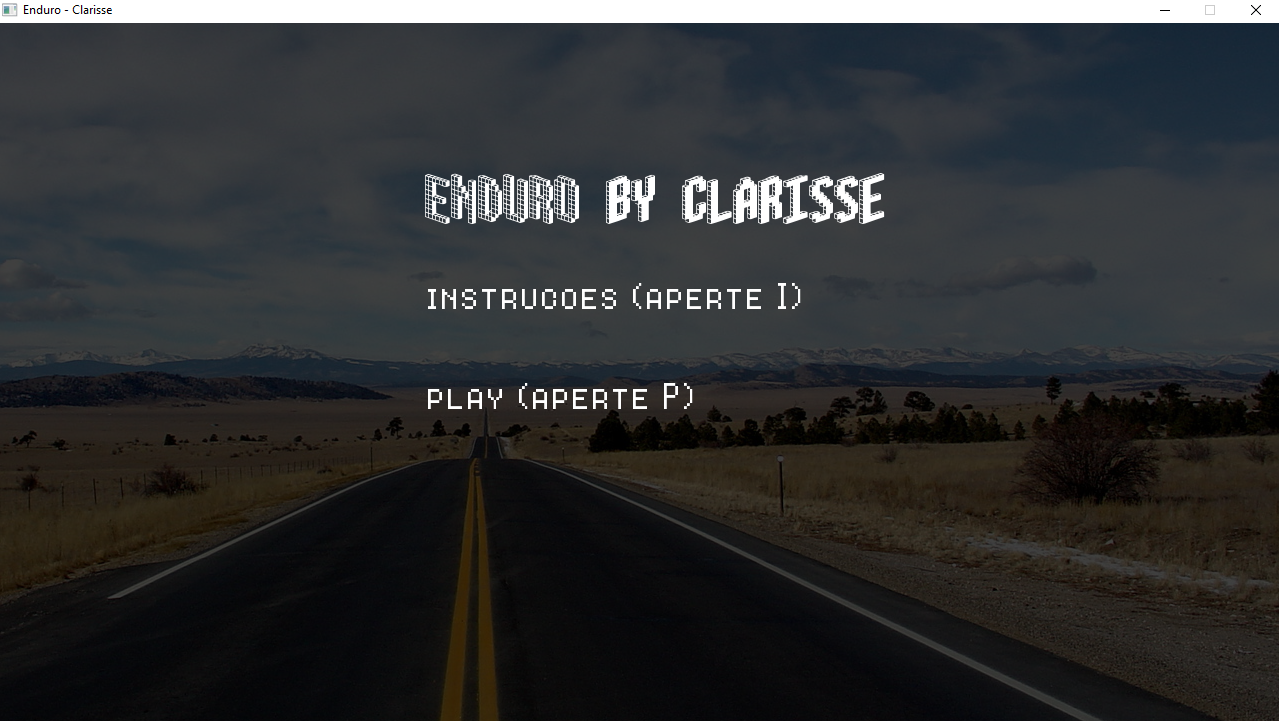
\includegraphics[width=0.8\textwidth]{menutela.png}
\caption{Tela inicial}
\end{figure}


    \begin{figure}[H]
    \centering
    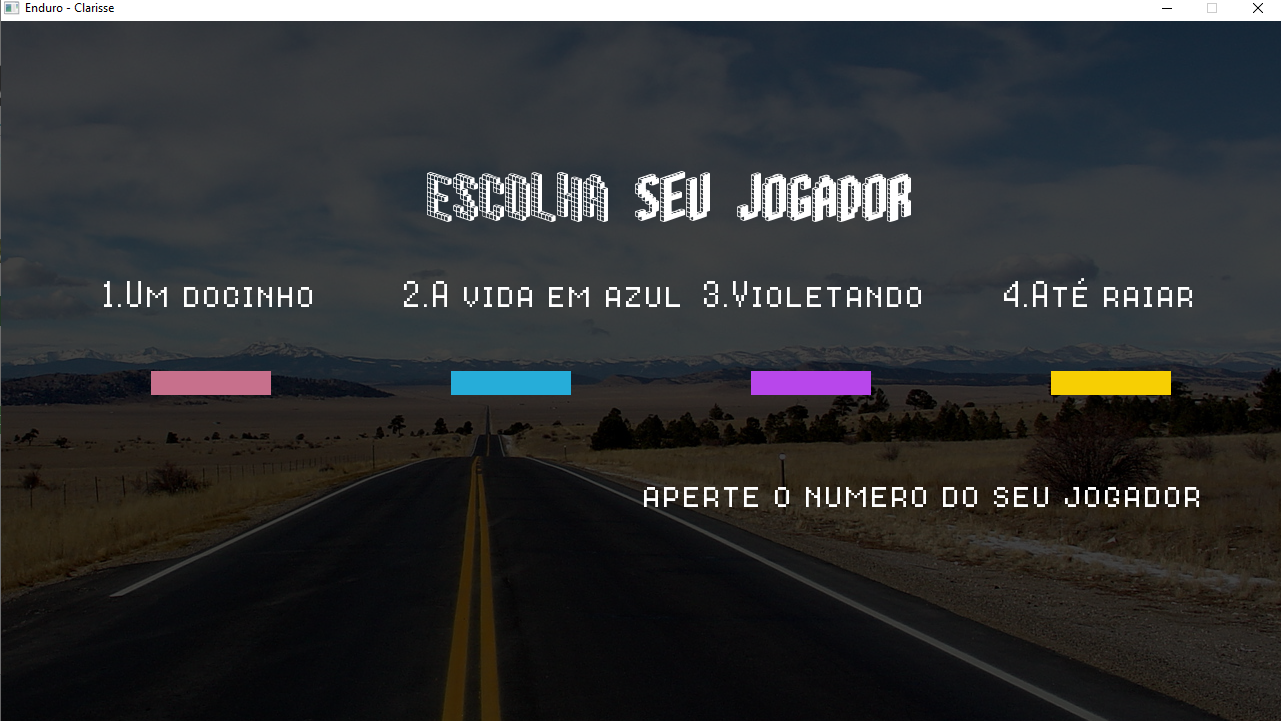
\includegraphics[width=0.8\textwidth]{menuplay.png}
    \caption{Tela }
    \end{figure}


\subsection{Conclusão}








\end{document}
